\section{Conics}

Conics are the geometric shapes formed by the intersection of a cone and a plane. 
These shapes include circles, ellipses, parabolas, and hyperbolas, as illustrated in the figure below:
\begin{figure}[H]
    \centering
    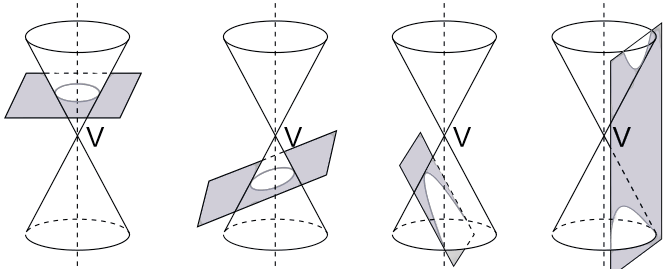
\includegraphics[width=0.5\linewidth]{images/conics.png}
\end{figure}
\begin{definition}[\textit{Conic}]
    A point $\mathbf{x}$  lies on a conic $\mathbf{C}$ if it satisfies the homogeneous quadratic equation $\mathbf{x}^TC\mathbf{x}=0$, where $\mathbf{C}$ is a symmetric matrix, a standard convention in defining conics.
\end{definition}
Conics are curves that can be described by second-degree equations in the plane. 
In Euclidean coordinates, a conic is expressed as:
\[ax^2+bxy+cy^2+dx+ey+f=0\]
In homogeneous coordinates, this equation becomes:
\[ax^2+bxy+cy^2+dxw+eyw+fw^2=0\]
Alternatively, conics can be represented in matrix form as:
\[\mathbf{x}^T \begin{bmatrix} a & \frac{b}{2} & \frac{d}{2} \\ \frac{b}{2} & c & \frac{e}{2} \\ \frac{d}{2} & \frac{e}{2} & f \end{bmatrix} \mathbf{x}=0\]
Conics have five degrees of freedom, meaning that five points are sufficient to uniquely determine a conic.
\begin{example}
    A circle in Cartesian coordinates is represented as:
    \[(x-x_0)^2+(y-y_0)^2-r^2=0\]
    In homogeneous coordinates, it is given by:
    \[\begin{bmatrix} x & y & w \end{bmatrix} \begin{bmatrix} 1 & 0 & -x_0 \\ 0 & 1 & -y_0 \\ -x_0 & -y_0 & x_0^2+y_0^2-r^2 \end{bmatrix} \begin{bmatrix} x \\ y \\ w \end{bmatrix} = 0\]
\end{example}

When a conic is represented by a quadratic equation and a line by a linear equation, their intersection results in a second-degree equation in the point $\mathbf{x}$. 
Therefore, a line and a conic always intersect at two points, which can be categorized as follows:
\begin{itemize}
    \item \textit{Real and distinct}: two separate real points.
    \item \textit{Real and coincident}: one real point, a repeated or double root.
    \item \textit{Complex and distinct}: two distinct complex conjugate points.
    \item \textit{Complex and coincident}: one complex point, a repeated or double root.
\end{itemize}
This is due to the fundamental theorem of algebra, which guarantees two solutions to a second-degree equation when considering complex numbers.
\begin{figure}[H]
    \centering
    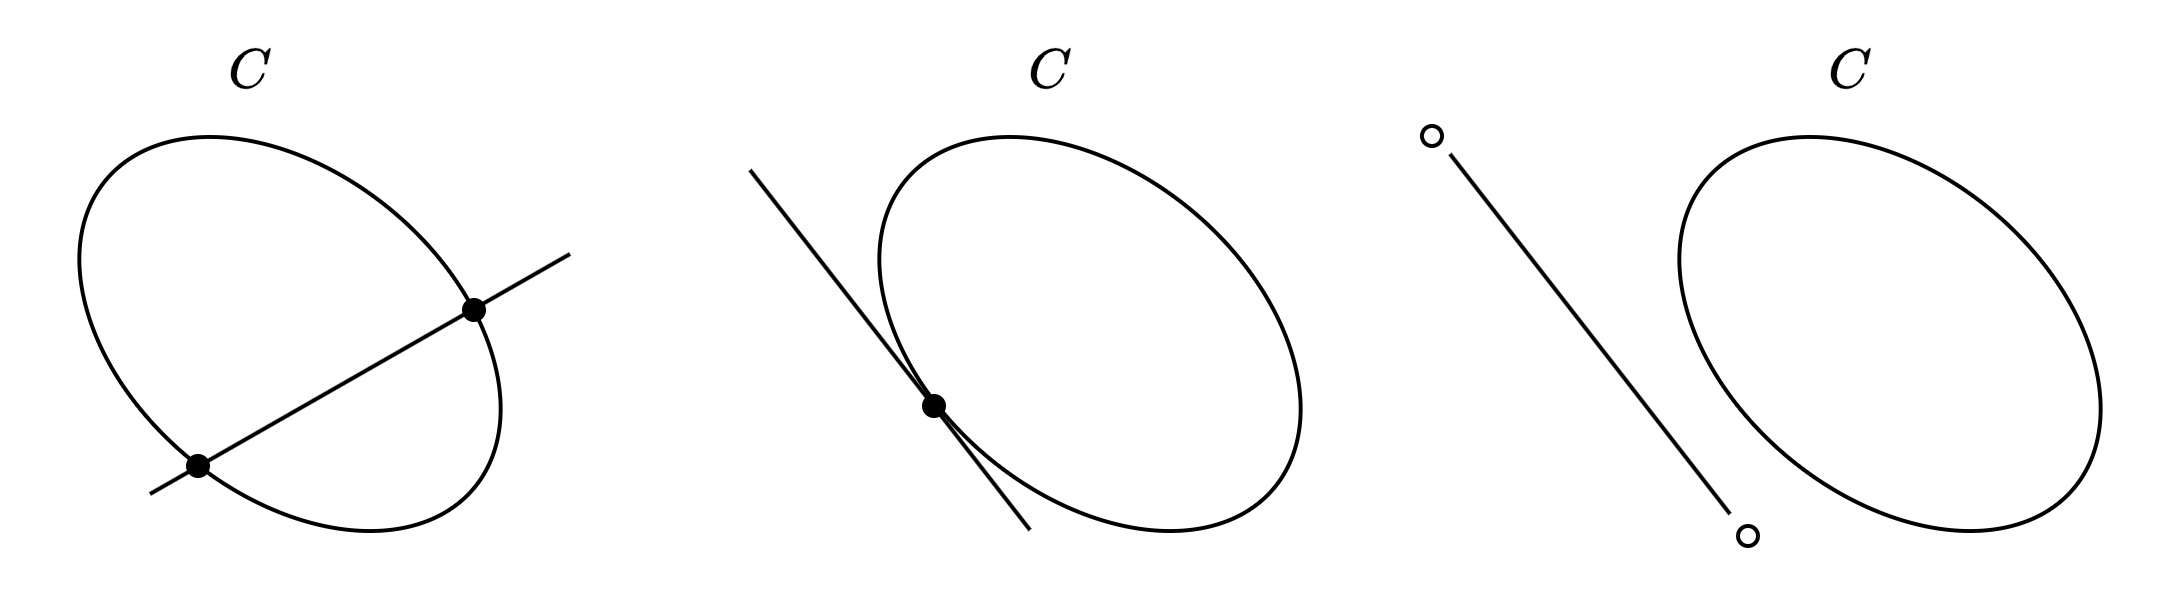
\includegraphics[width=0.75\linewidth]{images/intersection.png}
    \caption{Intersection with two real roots, two coincident roots and two imaginary roots}
\end{figure}
The intersection of the line at infinity with a conic yields the following results:
\begin{itemize}
    \item \textit{Parabola}: two coincident solutions, representing the point at infinity along the axis.
    \item \textit{Ellipse}: two complex-conjugate solutions, indicating no real solutions.
    \item \textit{Hyperbola}: two real and distinct solutions, corresponding to the asymptotes.
\end{itemize}

\subsection{Circular points}
\begin{example}
    When a circle is intersected with the line at infinity, the system becomes:
    \[\begin{cases}
        x^2-2x_0w+x_0^2w^2+y^2-2y_0w+y_0^2w^2-r^2w^2=0 \\
        w=0
    \end{cases}\]
    This simplifies to:
    \[x^2+y^2=0\]
    Here, the parameters of the circle (center and radius) disappear, indicating that the two intersection points are the same for all circles.
\end{example}
\begin{definition}[\textit{Circular points}]
    The two intersection points obtained by intersecting any circle with the line at infinity are called the circular points. 
    These points are:
    \[\mathbf{I}=\begin{bmatrix} 1 \\ i \\ 0 \end{bmatrix} \qquad \mathbf{J}=\begin{bmatrix} 1 \\ -i \\ 0 \end{bmatrix}\]
\end{definition}

\subsection{Polar line}
\begin{definition}[\textit{Polar line}]
    Given a point $\mathbf{y}$ and a conic $\mathbf{C}$, the line $\mathbf{l}=\mathbf{Cy}$ is called the polar line of the point $\mathbf{y}$ with respect to the conic $\mathbf{C}$. 
\end{definition}
\begin{figure}[H]
    \centering
    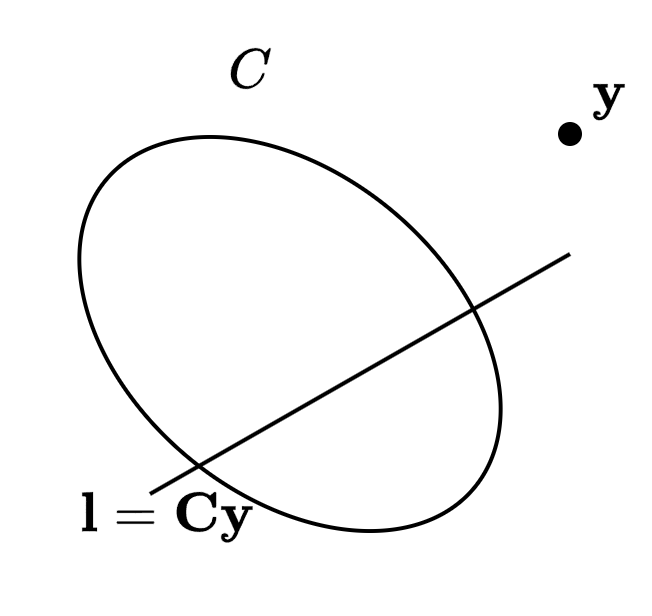
\includegraphics[width=0.3\linewidth]{images/polar.png}
    \caption{Polar line}
\end{figure}

\subsection{Harmonic tuples}
\begin{definition}[\textit{Harmonic tuple}]
    A 4-tuple of collinear points $\mathbf{a}, \mathbf{b}, \mathbf{c}, \mathbf{d}$ is called a harmonic tuple if their cross ratio is equal to $-1$.
\end{definition}
A harmonic cross ratio value is shared by other collinear 4-tuples. 
A common example is:
\[\left( \mathbf{y},\mathbf{z},\text{midPoint}(\mathbf{y},\mathbf{z}),P(\infty) \right)\]
Moreover, if $(\mathbf{a}, \mathbf{b}, \mathbf{c}, \mathbf{d})$ is harmonic, then $(\mathbf{c}, \mathbf{d}, \mathbf{a}, \mathbf{b})$ is also harmonic. 
\begin{definition}[\textit{Conjugate points}]
    In a harmonic tuple $(\mathbf{a}, \mathbf{b}, \mathbf{c}, \mathbf{d})$, the points $\mathbf{a}$ and $\mathbf{b}$ are said to be conjugate with respect to $\mathbf{c}$ and $\mathbf{d}$.
\end{definition}
Since the cross ratio of a harmonic tuple is negative, conjugate points $\mathbf{a}$ and $\mathbf{b}$ lie on opposite sides of the segment formed by $\mathbf{c}$ and $\mathbf{d}$, with one point inside and the other outside the segment.

\subsection{Polar line and harmonic tuples}
Given any point $\mathbf{z}$ on the polar line $\mathbf{l}=\mathbf{Cy}$, consider the line passing through the points $\mathbf{y}$ and $\mathbf{z}$. 
Let $\mathbf{x}_1$ and $\mathbf{x}_2$ represent the points at which this line intersects the conic $\mathbf{C}$. 
\begin{figure}[H]
    \centering
    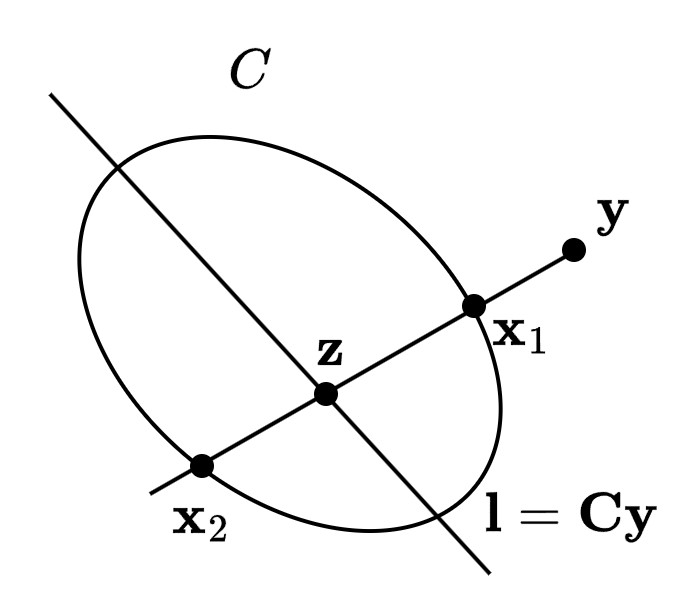
\includegraphics[width=0.25\linewidth]{images/polarharmonic.png}
\end{figure}
\begin{theorem}
    If $\mathbf{x}_1$ and $\mathbf{x}_2$ are the points where the line passing through $\mathbf{y}$ and $\mathbf{z}$ intersects the conic $\mathbf{C}$, then $\mathbf{y}$ and $\mathbf{z}$ are conjugate with respect to $\mathbf{x}_1$ and $\mathbf{x}_2$.
\end{theorem}
The polar line $\mathbf{l}=\mathbf{Cy}$ contains all points that are conjugate to $\mathbf{y}$ with respect to the conic $\mathbf{C}$. 
Specifically, it includes points that are conjugate with respect to the intersection points of $\mathbf{C}$ with any line passing through $\mathbf{y}$.

\subsection{Polar line and tangency points}
As the line through $\mathbf{y}$ approaches tangency with the conic $\mathbf{C}$, the points $\mathbf{x}_1$ and $\mathbf{x}_2$ merge into the point of tangency. 
Consequently, the conjugate point $\mathbf{z}$ also coincides with the tangency point, applying to any line tangent to $\mathbf{C}$ from point $\mathbf{y}$.

Therefore, the polar line $\mathbf{l}=\mathbf{Cy}$ passes through the tangency points where lines from $\mathbf{y}$ meet the conic $\mathbf{C}$.
If a point $\mathbf{z}$ lies on the conic, $\mathbf{y}$ is one of its conjugates with respect to the same conic. 
The tangent line $\mathbf{lz}$ to the conic at point $\mathbf{z}$ contains points conjugate to $\mathbf{z}$, making $\mathbf{lz}$ the polar line of $\mathbf{z}$ with respect to the conic.
\begin{figure}[H]
    \centering
    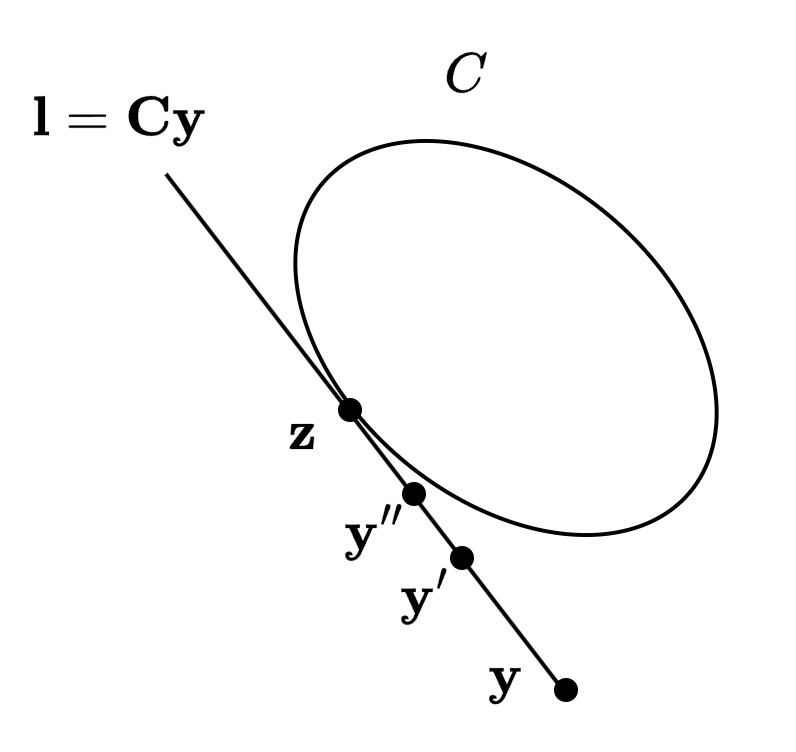
\includegraphics[width=0.4\linewidth]{images/tangentpolar.png}
\end{figure}
In the illustration, the polar line $\mathbf{lz}=\mathbf{Cz}$ for point $\mathbf{z}$ on the conic $\mathbf{C}$ corresponds to the tangent line to the conic at point $\mathbf{z}$.
\begin{example}
    Consider a circle with radius $r$ centered at the origin and the point $\mathbf{y}={\begin{bmatrix} x & 0 & 1 \end{bmatrix}}^T$. 
    The equation for the polar line is:
    \[\mathbf{l}=\mathbf{Cy}=\begin{bmatrix} 1 & 0 & 0 \\ 0 & 1 & 0 \\ 0 & 0 & -r^2 \end{bmatrix} \begin{bmatrix} \mathbf{x} \\ 0 \\ 1 \end{bmatrix} = \begin{bmatrix} \mathbf{x} \\ 0 \\ -r^2 \end{bmatrix}\]
    The Cartesian equation of the polar line becomes:
    \[\mathbf{x} x-r^2 = 0 \rightarrow x=\dfrac{r^2}{\mathbf{x}}\]
    This represents a vertical line.
\end{example}
From this, we deduce that the polar of a point $\mathbf{p}$ with respect to a circle is a line perpendicular to the line segment connecting the center of the circle to $\mathbf{p}$.
\begin{example}
    For a circle with radius $r$ centered at the origin and the point $\mathbf{y}={\begin{bmatrix} x & 0 & 0 \end{bmatrix}}^T$, the polar line equation is:
    \[\mathbf{l}=\mathbf{Cy} = \begin{bmatrix} 1 & 0 & 0 \\ 0 & 1 & 0 \\ 0 & 0 & -r^2 \end{bmatrix} \begin{bmatrix} \mathbf{x} \\ 0 \\ 0 \end{bmatrix} =  \begin{bmatrix} \mathbf{x} \\ 0 \\ 0 \end{bmatrix}\]
    The Cartesian equation becomes:
    \[\mathbf{x} x=0 \rightarrow \mathbf{x}=0\]
    This equation describes the diameter of the circle perpendicular to the direction of $\mathbf{y}$.
\end{example}
Parallel tangent lines from a point at infinity will have tangency points lying along a diameter that is perpendicular to the direction of the tangents.
\begin{figure}[H]
    \centering
    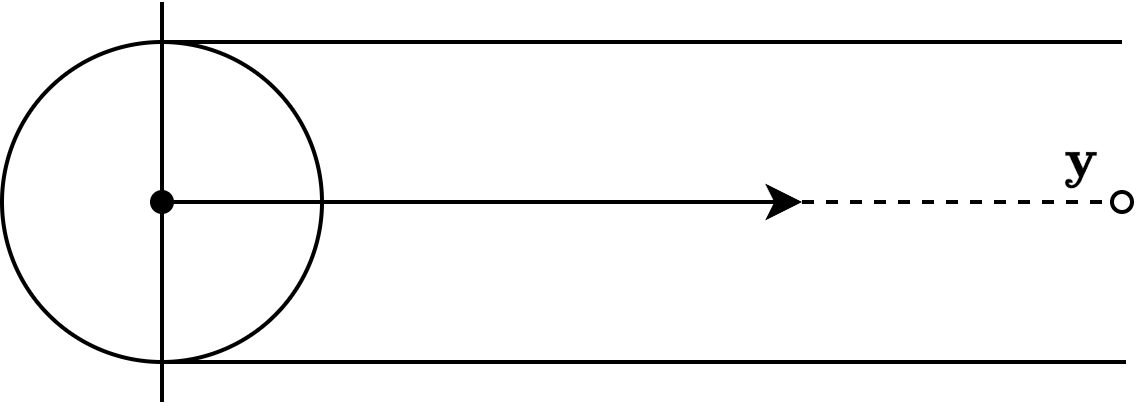
\includegraphics[width=0.5\linewidth]{images/parallel.png}
\end{figure}
\begin{example}
    For a circle with radius $r$ centered at the origin and the point $\mathbf{y}={\begin{bmatrix} x & 0 & 0 \end{bmatrix}}^T$, the polar line equation is:
    \[\mathbf{l}=\mathbf{Cy}=\begin{bmatrix} 1 & 0 & 0 \\ 0 & 1 & 0 \\ 0 & 0 & -r^2 \end{bmatrix}\begin{bmatrix} 0 \\ 0 \\ 1 \end{bmatrix} = \begin{bmatrix} 0 \\ 0 \\ -r^2 \end{bmatrix}\]
    The Cartesian equation becomes:
    \[-r^2w=0 \rightarrow \mathbf{x}=0\]
    This equation describes the line at infinity. 
\end{example}
\begin{property} 
    The polar line of any point at infinity is a diameter. 
\end{property} 
\begin{property} 
    Any diameter passes through the center of the circle. 
\end{property} 
\begin{property} The center is conjugate to every point at infinity.
\end{property} 
\begin{property}
    All points at infinity are conjugate to the center. 
\end{property} 
\begin{property} The polar of the center is the line that includes all points at infinity. 
\end{property} 
\begin{property}
    The polar line of the center is the line at infinity. 
\end{property}

\subsection{Degenerate conics}
\begin{definition}[\textit{Non-degerate conic}]
    A non-degenerate conic has a non-singular matrix $\mathbf{C}$, meaning:
    \[\textnormal{rank}(\mathbf{C})=3\]
\end{definition}
\begin{definition}[\textit{Degerate conic}]
    A degenerate conic has a singular matrix $\mathbf{C}$, meaning:
    \[\textnormal{rank}(\mathbf{C}) < 3\]
\end{definition}
There are two types of degenerate conic: 
\begin{itemize}
    \item \textit{Rank 2}: when $\textnormal{rank}(\mathbf{C}) = 2$, $\mathbf{C}$ can be written as:
        \[\mathbf{C}=\mathbf{lm}^T+\mathbf{ml}^T\]
        Here, $\mathbf{x}$ satisfies $\mathbf{x}^T \mathbf{Cx} = 0$ when either $\mathbf{x}^T \mathbf{l} = 0$ or $\mathbf{m}^T \mathbf{x} = 0$, meaning $\mathbf{x}$ lies on the union of lines $\mathbf{l}$ and $\mathbf{m}$.
        \begin{figure}[H]
            \centering
            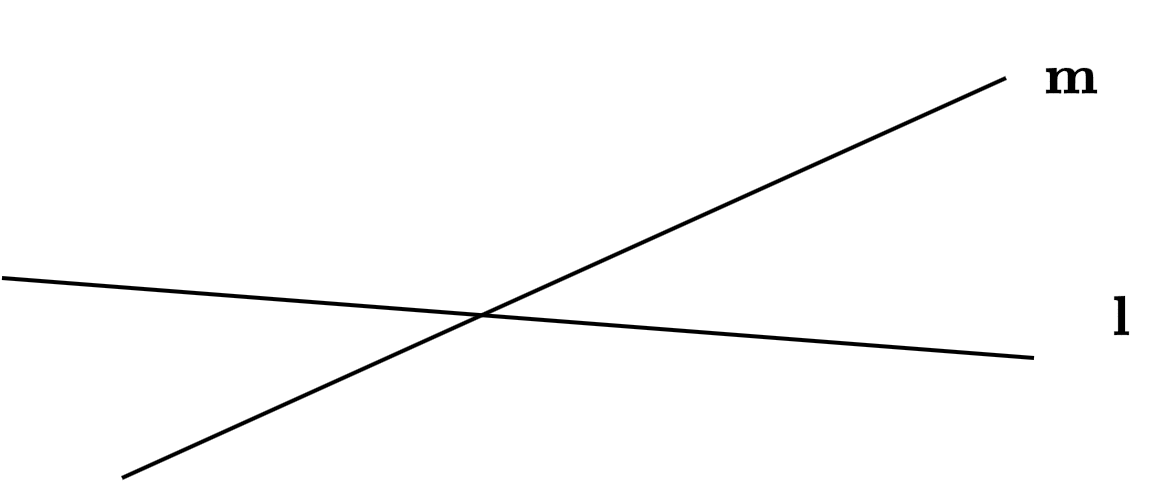
\includegraphics[width=0.35\linewidth]{images/inters.png}
        \end{figure}
    \item \textit{Rank 1}: when $\textnormal{rank}(\mathbf{C}) = 1$, $\mathbf{C}$ can be written as:
        \[\mathbf{C}=\mathbf{ll}^T\]
        The conic consists of points $\mathbf{x}$ that satisfy $\mathbf{x}^T \mathbf{Cx} = 0$, meaning $\mathbf{x}$ lies on the repeated line $\mathbf{l}$.
        \begin{figure}[H]
            \centering
            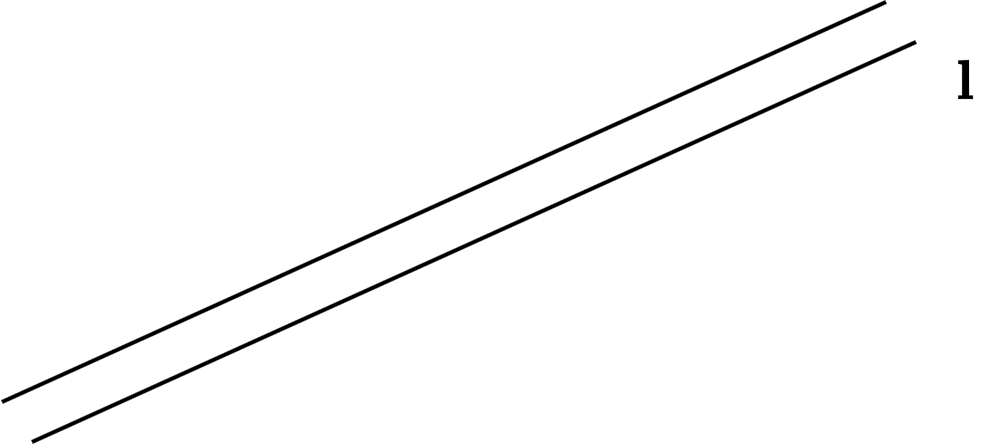
\includegraphics[width=0.35\linewidth]{images/rep.png}
        \end{figure}
\end{itemize}